\section{Implementácia ovládača}
\label{sec:program}

\begin{figure}[!htbp]
	\begin{center}
		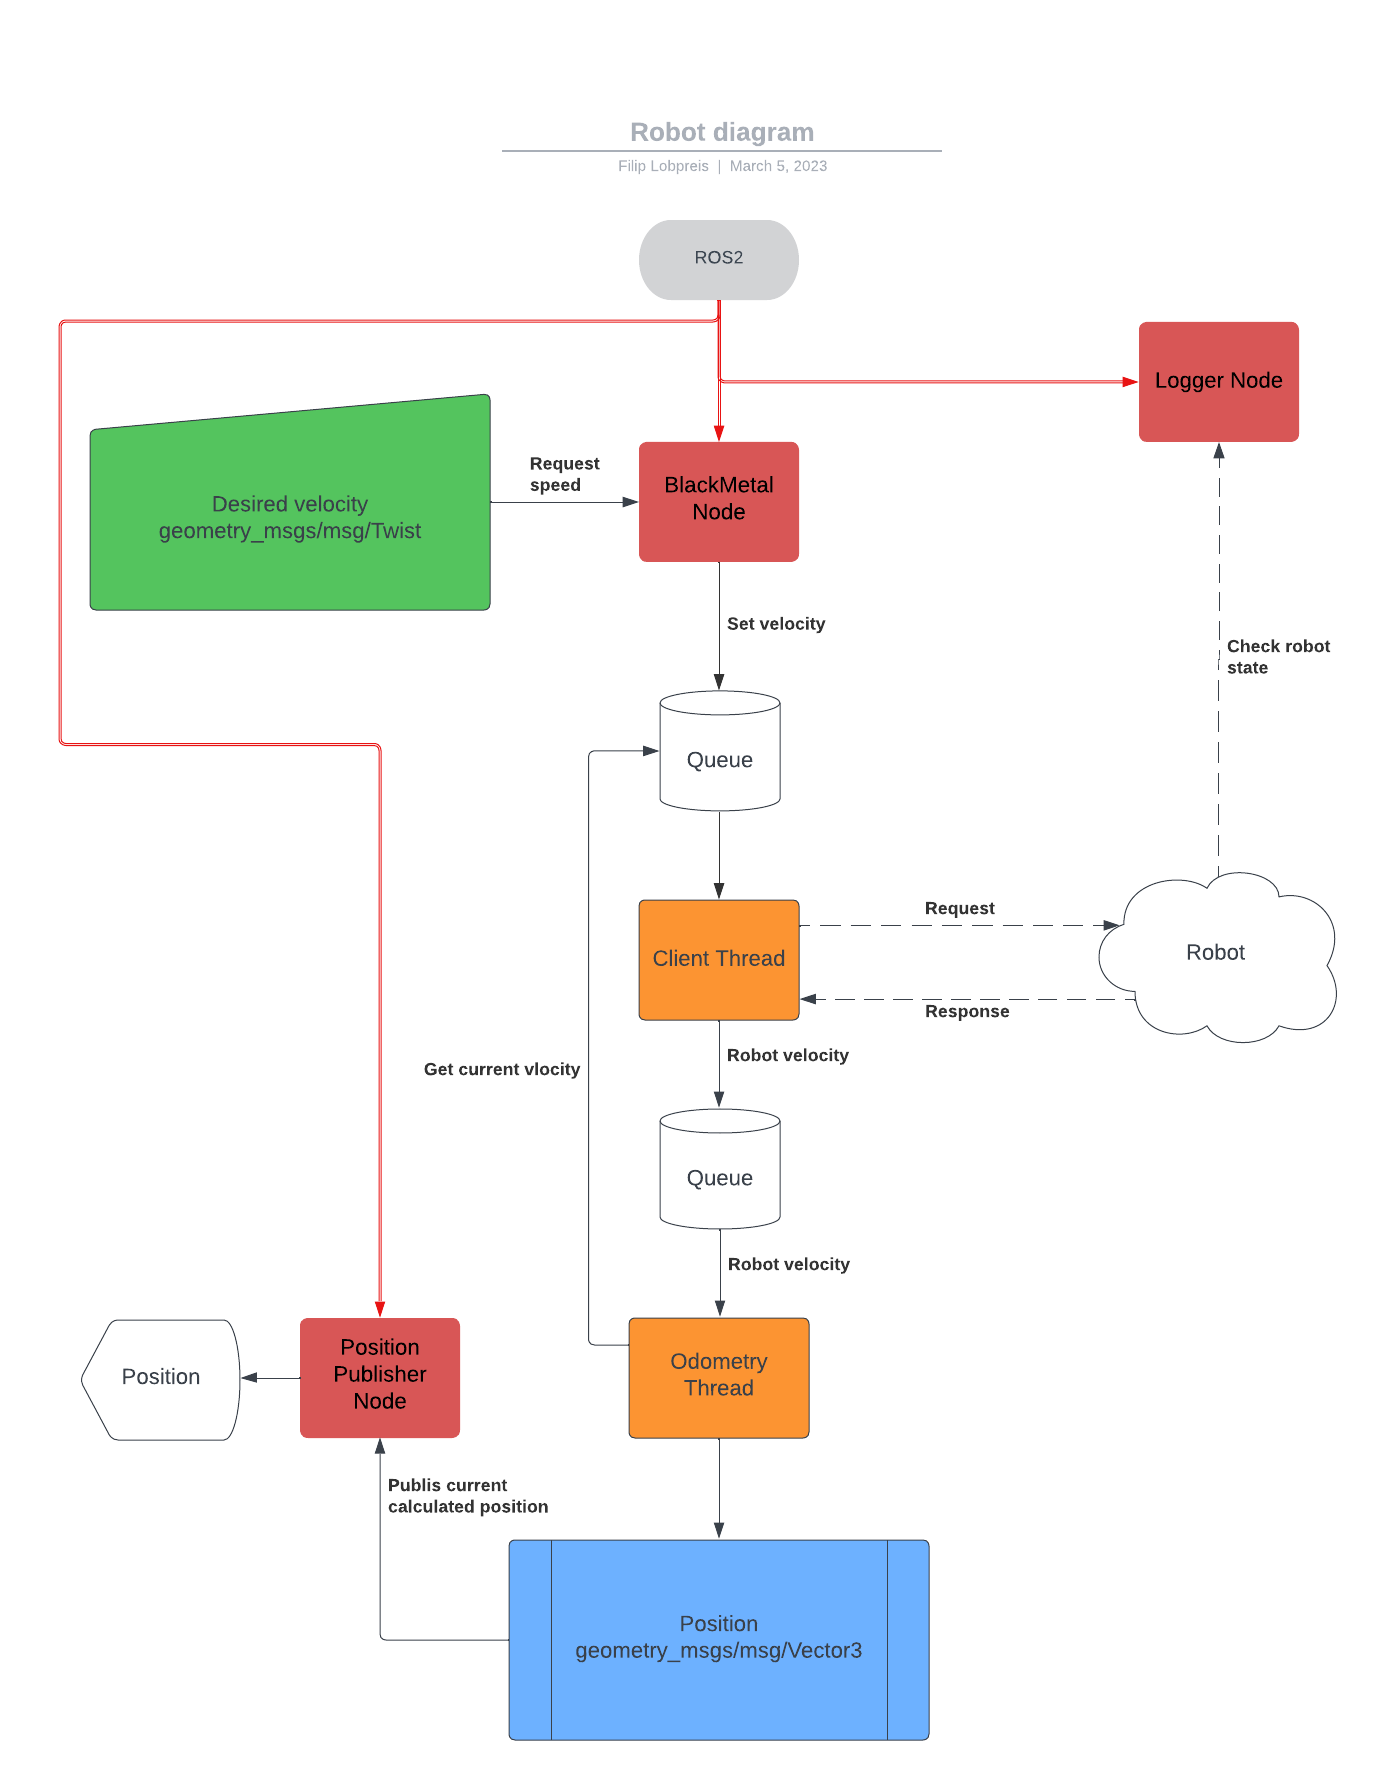
\includegraphics[width=0.9\textwidth]{img/BlackMetal_flowchart.png}
	\end{center}
	\caption{Graf vykonávania programu na~ovládanie robota pomocou ROS2.}
	\label{fig:flowchart}
\end{figure}

\subsection{Úvod do~čítania grafu}
\label{sec:citanie_grafu}

Na~obrázku Obr.~\ref{fig:flowchart} môžeme vidieť viacero objektov rôznych farieb. Objekty zobrazené červenou farbou sú uzly spracovávané
a~vytvárané v~rámci ROS2. Každý tento objekt sa vykonáva v~osobitnom procese. Objekty zobrazené oranžovou farbou sú objekty, ktoré majú svoje
vlastné vlákno. Tieto objekty boli vytvorené uzlom BlackMetal. Dátové štruktúry Queue, zobrazené bielou farbou sú vytvorene  tak~aby
zabezpečovali bezchybnú komunikáciu medzi viacerými vláknami. Objekt so zelenou farbou je vstup do~programu. Je zadávaný užívateľom
a~reprezentuje žiadanú rýchlosť robota. Modry objekt je výstupom programu. Je to téma, na~ktorý sa publikuje aktuálna pozícia robota.
Robot samotný je zobrazený bielou farbou vo~forme malého obláčika. Prerušované čiary na~diagrame znázorňujú sieťovú komunikáciu programu
a~robota. Červené dvojité čiary udávajú, ktoré objekty patria ROS-u. Nakoniec čierne plné čiary reprezentujú tok dát medzi objektami.

\subsection{Uzly}

Na~obrázku Obr.~\ref{fig:flowchart} môžeme vidieť postup vykonávania programu na~ovládanie robota BlackMetal pomocou ROS2.
Na~začiatku programu sa vytvoria 3 uzly. Prvý uzol \textbf{Position Publisher Node} je uzol, na~ktorý sa publikuje vypočítaná pozícia robota.
Počíta sa na~základe obdržaných dát z~enkóderov robota. Uzol \textbf{Logger Node} slúži na~zaznamenávanie stavu robota \ref{sec:logovanie}.
Posledný uzol \textbf{BlackMetal Node} ovláda robota na~základe zadaných dát užívateľom.

\subsection{Vstup}

Uzol \textit{BlackMetal Node} vytvorí príjemcu, ktorý počúva na~téme \textit{geometry\_msgs/msg/Twist}. Tento vstup je vo~forme príkazu
zadaného v~príkazovom riadku. Vyzerá nasledovne:

\lstset{language=bash,
	basicstyle=\ttfamily,
	keywordstyle=\color{blue}\ttfamily,
	stringstyle=\color{orange}\ttfamily,
	commentstyle=\color{green}\ttfamily,
	morecomment=[l][\color{magenta}]{\#},
	numberstyle=\color{red}
}

\label{requestCommand}
\begin{lstlisting}[language=bash]
	ros2 topic pub /cmd_vel geometry_msgs/msg/Twist
		"linear:
			x: 0.0,
			y: 0.0,
			z: 0.0,
		angular:
			x: 0.0,
			y: 0.0,
			z: 0.0" -1
\end{lstlisting}

Tento \hyperref[requestCommand]{príkaz} publikuje jednu správu (\textit{-1}) o lineárnych a~uhlových rýchlostiach na~tému \textit{/cmd\_vel}
Táto sprava je typu \textit{geometry\_msgs/mgs/Twist}. Je následne spracovaná a~uložená do~rady \textit{Queue}. Tato rada je prioritne založená.
To znamená, že~požiadavka s nižším kódom ma vyššiu prioritu. Požiadavky a~ich kódy moceme vidieť v~sekcii \ref{sec:ovladanie}.

\subsection{Komunikacia s robotom}
\label{sec:robotComms}

Ako je naznačené na~Obr.~\ref{fig:flowchart}, klient si vo~svojom vlastnom vlákne vytiahne prvú spravu z~rady a~pretransformuje ju do~formy JSON.
Tento typ spravy môžeme vidieť v~\ref{sec:ovladanie}. Príkaz je poslaný robotu a~ten obratom dá vedieť, či danú požiadavku obdržal. Ak tato správa
žiadala rýchlosti kolies, tak~robot ďalšou správou odpovie na~danú požiadavku. Typ tejto odpovede môžeme vidieť v~\ref{jsonWannabeSpeed}. V~tomto prípade
sa správa spracuje a~uloží sa do~ďalšej rady.

\subsection{Odometria}
\label{sec:odometria}

Odometria, počítanie polohy na~základe rýchlosti kolies, sa vykonáva rovnako ako komunikácia s robotom v~separátnom vlákne. Tu je potreba si uvedomiť
jednu skutočnosť. To je tá, že~keď posielame žiadosť na~nastavenie rýchlostí kolies robota, tak~robot si hodnoty v~žiadosti prepočíta a~dáta dá následne
enkóderov. Keď si ale tieto rýchlosti vyžiadame z~enkóderov, tak~sa robot týchto dát nechytá a~my si ich musíme prepočíta na~metre za sekundu. Zároveň
si tento objekt neustále pýta od robota rýchlosti kolies. Ako sme už spomenuli v~\ref{sec:robotComms}, tieto spravy majú nižšiu prioritu ako nastavenie
rýchlosti kolies alebo bezpečnostné zastavenie robota. Preto sa môže stat, že~správy posielané robotu nebudú dodržiavať presne stanovenú frekvenciu v~čase
keď mu bude užívateľ posielať príkazy.

\subsection{Zdieľanie polohy}
\label{sec:zdielanie_polohy}

Ďalšiu vec, ktorú je treba vysvetliť ku grafu Obr.~\ref{fig:flowchart} je zdieľanie polohy. Odometria po~každom prepočítaní polohy robota publikuje tuto
informáciu na~tému \textit{/position} tato sprava je typu \textit{geometry\_msgs/msg/Vector3}. Obsahuje 3 hodnoty, ktoré sú x, y a~z.
Súradnice reprezentujú aktuálnu polohu robota.

